% Created 2020-09-10 Thu 02:11
% Intended LaTeX compiler: lualatex
\documentclass[11pt]{article}
\usepackage{graphicx}
\usepackage{grffile}
\usepackage{longtable}
\usepackage{wrapfig}
\usepackage{rotating}
\usepackage[normalem]{ulem}
\usepackage{amsmath}
\usepackage{textcomp}
\usepackage{amssymb}
\usepackage{capt-of}
\usepackage{hyperref}
\usepackage{tabularx}
\usepackage{etoolbox}
\makeatletter
\def\dontdofcolorbox{\renewcommand\fcolorbox[4][]{##4}}
\AtBeginEnvironment{minted}{\dontdofcolorbox}
\makeatother
\usepackage[newfloat]{minted}
\usepackage{amsthm}
\theoremstyle{definition}
\newtheorem{definition}{Definition}[section]
\usepackage{unicode-math}
\usepackage{unicode}
\author{Mark Armstrong}
\date{Fall 2020}
\title{Introduction and overview\\\medskip
\large Principles of Programming Languages}
\hypersetup{
   pdfauthor={Mark Armstrong},
   pdftitle={Introduction and overview},
   pdfkeywords={},
   pdfsubject={An introduction and a brief overview of topics we will discuss in the course.},
   pdfcreator={Emacs 27.0.90 (Org mode 9.3.7)},
   pdflang={English},
   colorlinks,
   linkcolor=blue,
   citecolor=blue,
   urlcolor=blue
   }
\begin{document}

\maketitle

\section{Preamble}
\label{sec:org78ddc8d}
The preamble section of each notes will include
\begin{itemize}
\item notable references,
\begin{itemize}
\item i.e., specific chapters of our recommended/additional texts
from which the notes are derived, or which expand on the notes,
\end{itemize}
\item a table of contents, and
\item an update history, chronicling any major changes.
\begin{itemize}
\item Note the git commit history will provide a more fine-grained
record of upates.
\end{itemize}
\end{itemize}

\subsection{{\bfseries\sffamily TODO} Notable references}
\label{sec:org534e54f}
:TODO:

\subsection{{\bfseries\sffamily TODO} Table of contents}
\label{sec:org3c3dc4d}
\begin{scriptsize}
\begin{itemize}
\item \hyperref[sec:org78ddc8d]{Preamble}
\end{itemize}
\end{scriptsize}

\section{Introduction}
\label{sec:org192cf72}
This section of notes introduces the course and the staff,
and lays out a few central concepts.

\section{Welcome}
\label{sec:org9b6f799}
\begin{center}
Welcome to the course!
\end{center}

\subsection{Instructor: Mark Armstrong}
\label{sec:orgf535182}
\begin{quote}
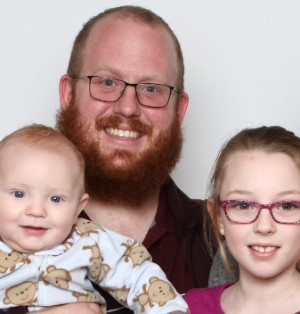
\includegraphics[width=200px]{./media/markarmstrong.jpg}
\end{quote}

\begin{itemize}
\item Email: \url{mailto:armstmp@mcmaster.ca}
\item Website: \url{https://armkeh.github.io}
\end{itemize}

\subsection{Teaching assistants}
\label{sec:orge8ec45e}
:TODO:

\section{Purpose and goals of this course}
\label{sec:orgf607cd6}
\subsection{Calendar description}
\label{sec:org4ea5367}
Design space of programming languages;
abstraction and modularization concepts and mechanisms;
programming in non-procedural (functional and logic) paradigms;
introduction to programming language semantics.

\subsection{Informal objectives}
\label{sec:org313558c}
\begin{itemize}
\item Investigate a number of programming languages
which exemplify different paradigms.
\begin{itemize}
\item A relatively shallow but comprehensive survey.
\item Focusing on general-purpose languages.
\end{itemize}
\item \emph{Formally} describe programming language syntax and semantics.
\begin{itemize}
\item An application of theory learned previously.
\end{itemize}
\item Apply various abstraction and modularisation techniques,
\begin{itemize}
\item Learning how to apply them and
to which situations they are best applied.
\end{itemize}
\end{itemize}

\subsection{Course preconditions}
\label{sec:org160979b}
Before beginning this course:

\begin{enumerate}
\item Students should know and understand:
a. Basic concepts about integers, sets, functions, \& relations.
b. Induction and recursion.
c. First order logic, axiomatic theories \& simple proof techniques.
d. Regular expressions \& context-free grammars.
e. Programming in imperative languages.
f. Basic concepts of functional programming languages.
\item Students should be able to:
a. Produce proofs involving quantifiers and/or induction.
b. Understand the meaning of a given axiomatic theory.
c. Construct regular sets \& context-free languages.
d. Produce small to medium scale programs in imperative languages.
e. Produce small scale programs in functional languages.
\end{enumerate}

\subsection{Course postconditions}
\label{sec:org55bc488}
After completion of this course:

\begin{enumerate}
\item Students should know and understand:
a. Programming in functional languages.
b. Programming in logical languages.
c. Formal definitions of syntax \& semantics for various
   simple programming languages.
d. Various abstraction \& modularisation techniques
   employed in programming languages.
\item Students should be able to:
a. Reason about the design space of programming languages,
   in particular tradeoffs \& design issues.
b. Produce formal descriptions of syntax \& semantics
   from informal descriptions, identifying ambiguities.
c. Select appropriate abstraction \& modularisation techniques
   for a given problem.
d. Produce tools for domain-specific languages
   in imperative, functional and logical languages.
\end{enumerate}

\subsection{Formal rubric for the course}
\label{sec:org05d35b3}
\begin{scriptsize}
\begin{center}
\begin{tabular}{|l|l|l|l|l|}
\hline
Topic & Below & Marginal & Meets & Exceeds \\
\hline
Familiarity & Shows some & Shows & Achieves & Achieves \\
with various & competence & competence & competence & competence \\
programming & in & in & with the & with \\
languages & procedural & procedural & basic & intermediate \\
 & languages, & languages & usage of & usage of \\
 & but not & and limited & various & various \\
 & languages & competence & languages & languages \\
 & from other & in & & \\
 & paradigms & languages & & \\
 & & from other & & \\
 & & paradigms & & \\
\hline
Ability to & Cannot & Identifies & Identifies & Identifies \\
identify and & consistently & such & such & sucj \\
make use of & identify & constructs, & constructs & constructs \\
abstraction, & such & but does not & and shows & and shows \\
modularisation & constructs & consistently & some ability & mastery of \\
constructs & & make use of & to make use & them when \\
 & & them when & of them when & programming \\
 & & programming & programming & \\
\hline
Ability to & Unable or & Comprehends & Makes only & Consistently \\
comprehend and & rarely & given & minor & fully \\
produce formal & able to & grammars, & errors & understands \\
descriptions & comprehend & but & regarding & given \\
of PL syntax & given & produces & precedence & grammars and \\
 & grammars; & grammars & or & produces \\
 & does not & which are & ambiguity & correct \\
 & identify & ambiguous & when & grammars. \\
 & ambiguity & or which do & reading or & \\
 & or & not & producing & \\
 & precedence & correctly & grammars & \\
 & rules & specify & & \\
 & & precedence & & \\
\hline
Ability to & Rarely or & Usually & Comprehends & Comprehends \\
comprehend and & never & comprehends & such & such \\
produce & comprehends & such semantic & semantic & semantic \\
operational & such & descriptions, & descriptions & descriptions \\
semantics for & semantic & but cannot & and produces & and produces \\
simple PLs & descriptions & consistently & them with & them without \\
 & & produce them & only minor & errors \\
 & & & errors & \\
\hline
\end{tabular}
\end{center}
\end{scriptsize}

\section{“Principles of programming languages”}
\label{sec:org7e487cb}
We begin the course with these fundamental questions.

\begin{itemize}
\item What is a \emph{programming language}?
\item What are the \emph{components} of a programming language?
\item How do we \emph{classify} a programming language?
\end{itemize}

\subsection{What is a programming language?}
\label{sec:orgf770cc7}

\begin{itemize}
\item A \emph{formal}, \emph{finitely described} language used for
describing (in most cases, potentially infinite) \emph{processes}.
\begin{itemize}
\item \emph{Formal} meaning described by a mathematical tool.
\begin{itemize}
\item Formality is necessary for a machine to understand the language.
\item Natural (human-spoken) languages are not formal.
\end{itemize}
\item A \emph{process} being some sequence of actions or steps.
\end{itemize}
\end{itemize}

\subsubsection{Example of a process}
\label{sec:org5f1ccbc}

Consider the mathematical function \(f(x) = x + 10\).
\begin{itemize}
\item On its own, this function is not a process;
\begin{itemize}
\item it is only a \emph{rule} that \(f(x)\) is related to \(x + 10\).
\end{itemize}
\end{itemize}

However, you likely learned as a child
a “program” describing the process for calculating \(f(x)\).
\begin{minted}[breaklines=true]{text}
start with all your fingers down
say “x” 
repeat until you run out of fingers:
  say the result of adding one to the number you just said
  put up one finger
the answer is the last number you said
\end{minted}

In computing, we sometimes conflate programs and (mathematical) functions.
\begin{itemize}
\item Sometimes, we must remember they are not the same.
\item Mathematical functions are rules. They do no computing.
\item Programs describe a sequences of steps.
They may tell us how to compute
the results of mathematical functions.
\end{itemize}

\subsection{What are the components of a programming language?}
\label{sec:org2c78087}

Just like a natural language, a programming language consists of
\begin{itemize}
\item \emph{syntactic} rules
\begin{itemize}
\item which describe the legal forms of programs, and
\end{itemize}
\item \emph{semantics} rules
\begin{itemize}
\item which describe the meaning of legal programs,
\begin{itemize}
\item if they in fact have a meaning!
\end{itemize}
\end{itemize}
\end{itemize}

\subsubsection{Syntax and semantics example}
\label{sec:org62d8d92}

For example, English syntax tells us a sentence structured
\begin{minted}[breaklines=true]{text}
adjective adjective (plural noun) (plural verb) adverb
\end{minted}
is grammatically correct.

In the same way, a Python compiler tells us a program of the form
\begin{minted}[breaklines=true]{python}
expression + expression
\end{minted}
is syntactically correct.

Note that in both cases, though, such sentences/programs
may be meaningless!
Noam Chomsky gave the example
\begin{quote}
Colourless green ideas sleep furiously.
\end{quote}

And we could construct the Python program
\begin{minted}[breaklines=true]{python}
1 + "hello"
\end{minted}
which crashes when run.

\subsubsection{Exercise: a meaningless C or Java program}
\label{sec:orgbf367d0}

Our example Python program above
\begin{minted}[breaklines=true]{python}
1 + "hello"
\end{minted}
is syntactically correct because Python is \emph{dynamically typed},
meaning that type errors such as this are not caught until runtime.

As an exercise, can you construct a similar example
of a program which is syntactically correct
but semantically meaningless in the \emph{statically typed} languages
C and Java?

Hint: consider using a value which does not have just one type.

\subsection{How do we classify a programming language?}
\label{sec:orgfc2da29}

First and foremost, we classify languages into \emph{paradigms},
\begin{itemize}
\item characterised by the set of \emph{abstractions} the language makes available.
\end{itemize}

But also in many other ways, such as:
\begin{itemize}
\item Typing properties, including
\begin{itemize}
\item static or dynamic (runtime) typechecking,
\item “weak” or “strong” typing discipline,
\item polymorphism support, builtin types, methods of defining new types, etc.
\end{itemize}
\item (Primary) implementation strategy: compiled or interpreted?
\item Ancestery or culture.
\begin{itemize}
\item “Scripting languages”
\item “JVM languages”
\item “The C-family”
\begin{itemize}
\item \url{https://en.wikipedia.org/wiki/List\_of\_C-family\_programming\_languages}
\end{itemize}
\end{itemize}
\end{itemize}

\section{Abstraction}
\label{sec:org1815e28}
:TODO:

\section{{\bfseries\sffamily TODO} Exercises}
\label{sec:org366191f}
\end{document}
